\section{Introducción}

Para este trabajo nos centraremos en resolver un problema real de aprendizaje automático utilizando el conocimiento obtenido a lo largo de las asignaturas de todo el Grado, con especial mención a los conocimientos adquiridos en las asignaturas \textit{Metaheurísticas} y \textit{Aprendizaje Automático}, y explorando nuevas técnicas de inteligencia artificial de cara a complementar dichos conocimientos de forma que se desarrolle un conocimiento en la exploración, formas de trabajo e investigación de nuevas técnicas.

\subsection{Problema a resolver}

En el año 1920 Thomas Wingate Todd publicó un artículo científico \cite{todd} en el que proponía una forma de clasificar en diez rangos de edad los restos óseos de una persona fallecida a partir de ciertas características de la sínfisis púbica, de forma que el proceso de identificación de cadáveres fuera más sencillo para los forenses.

A pesar de ser una publicación de hace más de cien años, este método sigue siendo la base para la estimación de la edad a partir de los restos óseos. La mayoría de técnicas actuales se basan en esta propuesta y se siguen aplicando de forma manual.

El sistema propuesto por Todd se centraba en nueve características, asignándole distintos valores categóricos, de la sínfisis púbica para realizar su clasificación:

\begin{enumerate}
	\item Crestas y surcos: Porosidad regular, muy definidas, poco profundas, restos de surcos o no hay surcos.
	\item Superficie porosa irregular: No, medianamente o sí.
	\item Borde superior: Definido o no definido.
	\item Nódulo óseo: Ausente o presente.
	\item Borde inferior: Definido o no definido.
	\item Borde dorsal: Definido o no definido.
	\item Plataforma dorsal: Ausente o presente.
	\item Bisel ventral: Ausente, en proceso de formación o formado.
	\item Borde ventral: Ausente, parcialmente formado, formado sin excrecencias, formado con pocas excrecencias o formado con muchas excrecencias.
\end{enumerate}

% Insertar PDF que paso sergio

% Please add the following required packages to your document preamble:
% \usepackage{graphicx}
\begin{table}[H]
\resizebox{\textwidth}{!}{%
	\begin{tabular}{|c|c|c|}
	\hline
	Crestas y surcos: Muy definidos & Superficie porosa irregular: Sí & Borde superior: Definido  \\ \hline
	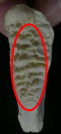
\includegraphics[scale = 0.75]{crestas_surcos_muy_definidos.png}  &   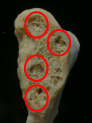
\includegraphics[scale = 0.75]{superficie_porosa_si.png} &  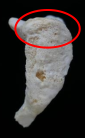
\includegraphics[scale = 0.75]{borde_superior_definido.png}  \\ \hline
	Nódulo óseo: Presente & Borde inferior: No definido & Borde dorsal: Definido \\ \hline
	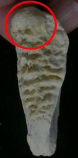
\includegraphics[scale = 0.75]{nodulo_oseo_presente.png} & 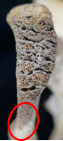
\includegraphics[scale = 0.75]{borde_inferior_no_definido.png} &  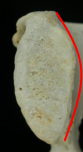
\includegraphics[scale = 0.75]{borde_dorsal_definido.png} \\ \hline
	Plataforma dorsal: Presente & Bisel ventral: En proceso de formación & Borde ventral: Muchas excrecencias \\ \hline
	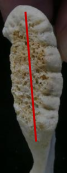
\includegraphics[scale = 0.75]{plataforma_dorsal_presente.png} & 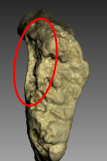
\includegraphics[scale = 0.75]{bisel_ventral_en_proceso_formacion.png} &   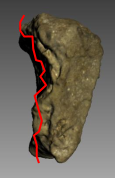
\includegraphics[scale = 0.75]{borde_ventral_muchas_excrecencias.png} \\ \hline
	\end{tabular}%
}
	\caption{Algunos ejemplos de las características consideradas por Todd.}\label{table:caracteristicas_todd}
\end{table}

\subsection{Motivación}

\subsection{Inteligencia Artificial Explicable}

En la última década, gracias a los avances en la potencia computación, los distintos modelos de aprendizaje automático como las redes neuronales han revolucionado la inteligencia artificial. Estos nuevos modelos, a pesar de obtener resultados impensables con modelos clásicos, son demasiado complejos como para comprender la forma en la que funcionan internamente. Por este motivo ha aparecido el concepto de Inteligencia Artificial Explicable \cite{XAI} (XAI de sus siglas en inglés).

La inteligencia artificial explicable trata de expresar modelos de inteligencia artificial de una forma simple e interpretable. Con esto se busca que no solo los desarrolladores de dichos modelos sean capaces de comprobar y validar como funciona el modelo, sino que los usuarios sean capaces de entender a grandes rasgos como funciona, ya que en muchas ocasiones han de ser capaces de interpretar las decisiones del modelo para realizar su trabajo.

En este trabajo, debido a la complejidad del problema, así como que el experto que utilizará los resultados del modelo ha de ser capaz de interpretar, validar, y tomar decisiones con los resultados del modelo, se buscará obtener un modelo simple y fácilmente interpretable.


\subsection{Objetivos}
